\section{Analysis}
\label{sec:analysis}

\subsection{Open sky}
\label{sec:open_sky}
This is the ideal condition measurement. The receiver is far from obstacles, it is not moving and the satellites are in line of sight so the signals are received directly. As we can see in figure \ref{fig:open_sky_fig_4} the best 50\% estimates are contained inside the circumference of a 3.2 meters radius, the number of satellites in view is stable at 8. The horizontal speed variation is at most 1 meter and the Horizontal Geometric Dilution of Precision (HDOP), which measures how the satellite geometry affects the accuracy of the horizontal position, is mostly stable at 1.03 (the lower the better).

\begin{figure}[H]
  \begin{subfigure}{.22\textwidth}
  \centering
    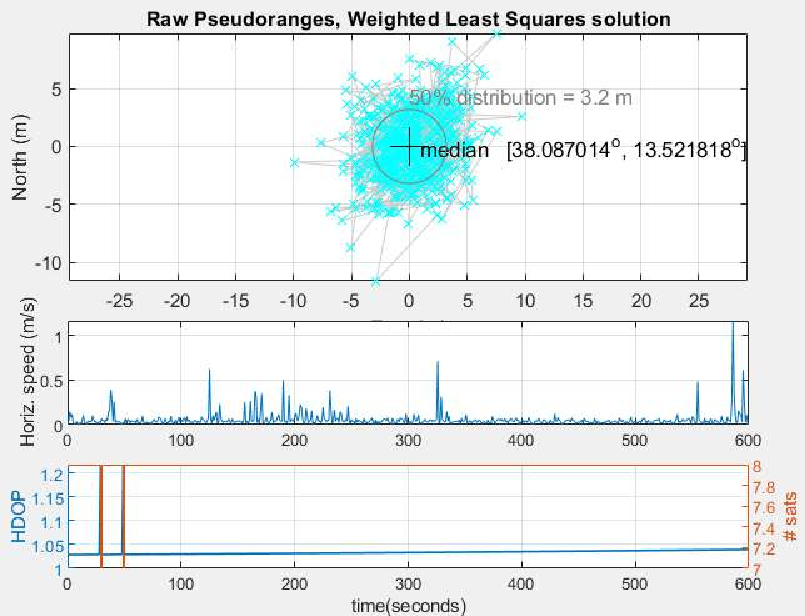
\includegraphics[width=1\linewidth]{images/open_sky_fig_4.pdf}
    \caption{Position estimate, Horizontal speed, HDOP}
    \label{fig:open_sky_fig_4}
  \end{subfigure}
  \begin{subfigure}{.22\textwidth}
  \centering
    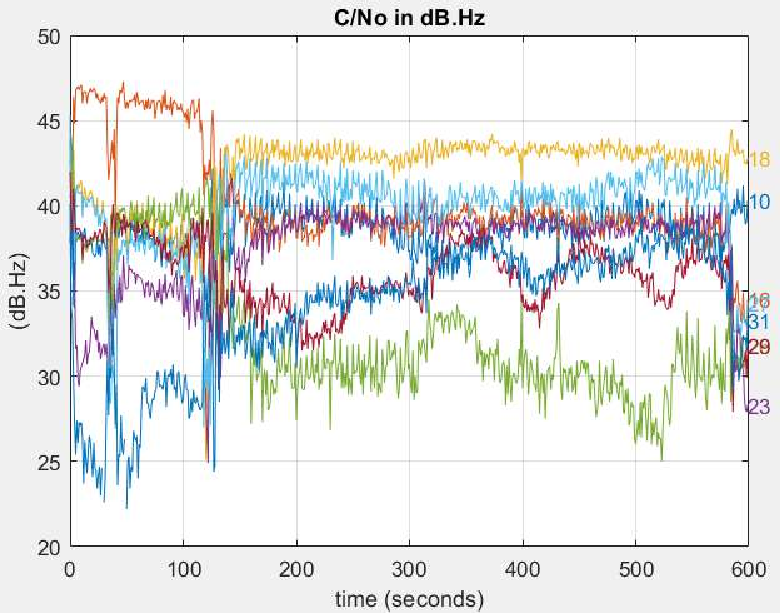
\includegraphics[width=1\linewidth]{images/open_sky_fig_3.pdf}
    \caption{C/N0 in dB.Hz}
    \label{fig:open_sky_fig_3}
  \end{subfigure}
  \vspace{10pt}
  %\caption{Positioning solution on map}
  %\captionsetup[subfigure]{position=below}
\end{figure}

\subsection{Indoor}
\label{sec:indoor}
This measurement was performed inside a building, so the satellites line of sigh is very limited. In figure \ref{fig:indoor_fig_4} we observe that the 50\% of the position estimates are contained in a circle with a radius of 30 meters, this result, as expected, is worse than the one in open sky condition. Moreover, the horizontal speed has 20 m/s peaks even if the receiver is not moving. The number of satellites in sight varies mostly between 3 and 6 and the HDOP is unstable and it's even 20 times higher with respect to open sky measurement, meaning a very bad satellite geometrical distribution. According to the figure \ref{fig:indoor_fig_3} the C/N0 has a mean value of 26.15 dB.Hz and a standard deviation of 4.31 dB.Hz so the signals of some satellites are not very stable. Overall the C/N0 is 30\% lower then the ideal condition measurement.
\begin{figure}[H]
  \begin{subfigure}{.22\textwidth}
  \centering
    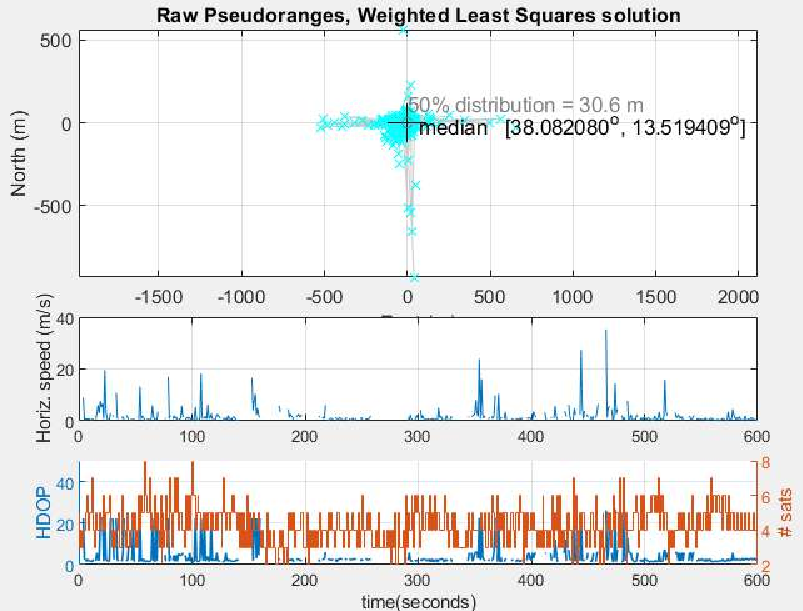
\includegraphics[width=1\linewidth]{images/indoor_fig_4.pdf}
    \caption{Position estimate, Horizontal speed, HDOP}
    \label{fig:indoor_fig_4}
  \end{subfigure}
  \begin{subfigure}{.22\textwidth}
  \centering
    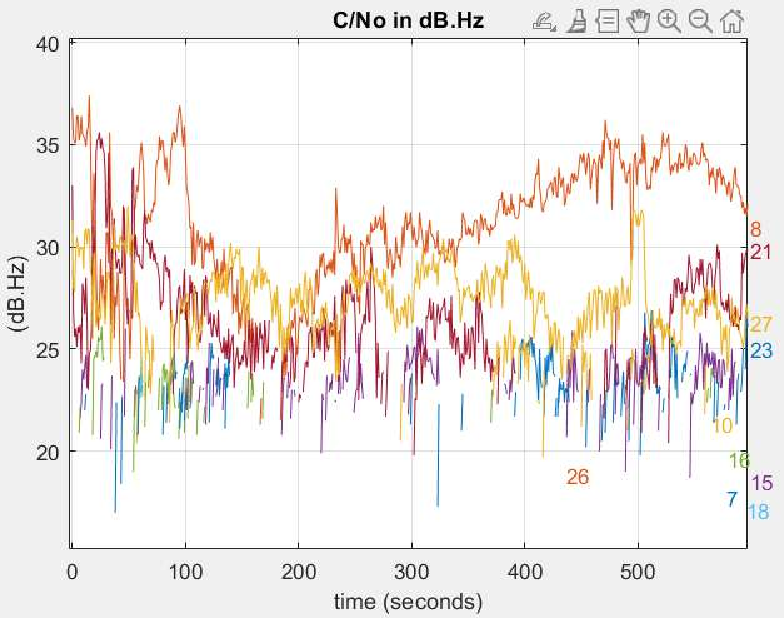
\includegraphics[width=1\linewidth]{images/indoor_fig_3.pdf}
    \caption{C/N0 in dB.Hz}
    \label{fig:indoor_fig_3}
  \end{subfigure}
  \vspace{10pt}
  %\caption{Simona sei falsa}
  %\captionsetup[subfigure]{position=below}
\end{figure}

\subsection{Walking}
\label{sec:walking}
For this measurement the receiver is moving and the line-of-sight is obstructed in certain moments, this depends on the chosen route because the receiver is not static, and if it's near obstacles, the signals may bounce around. The horizontal speed has some oscillations, which is expected due to the movement of the receiver, but there are some spikes around 14 m/s (but better than \ref{sec:indoor}) and this is an indicator of the accuracy of the measurement because it's not plausible for a human walking. As we can see in figure \ref{fig:figure4_walking} the number of satellites in sight is not stable, in certain instants it's even 1, this means that the position in those cases is not reliable because in order to obtain a correct position we need at least 4 satellites. HDOP has a mean value of 2.91 with a standard deviation of 3.92, and these elevated values contribute to increased errors in the estimated position. In figure \ref{fig:walking_figure_3.pdf} the carrier to noise density ratio has a mean value of 24.39 dB.Hz and a standard deviation of 5.87 dB.Hz, which is worse than the previous scenarios.
\begin{figure}[H]
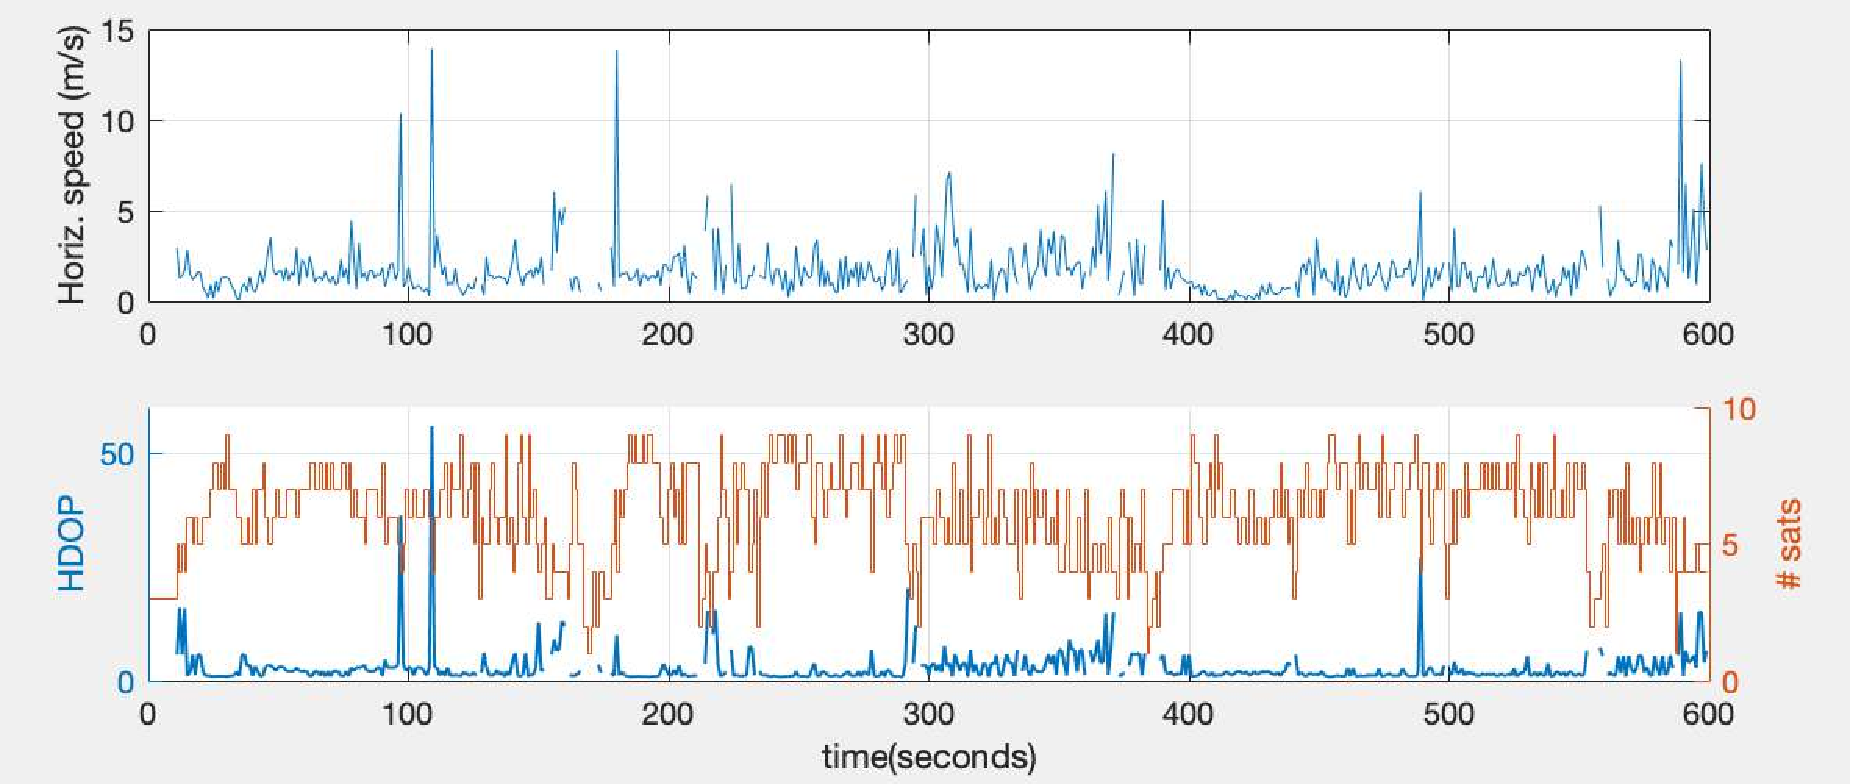
\includegraphics[scale=0.22]{images/walking_figure_4.pdf}
\caption{Horizontal speed and HDOP}
\label{fig:figure4_walking}
\end{figure}
%\begin{figure}[H]
%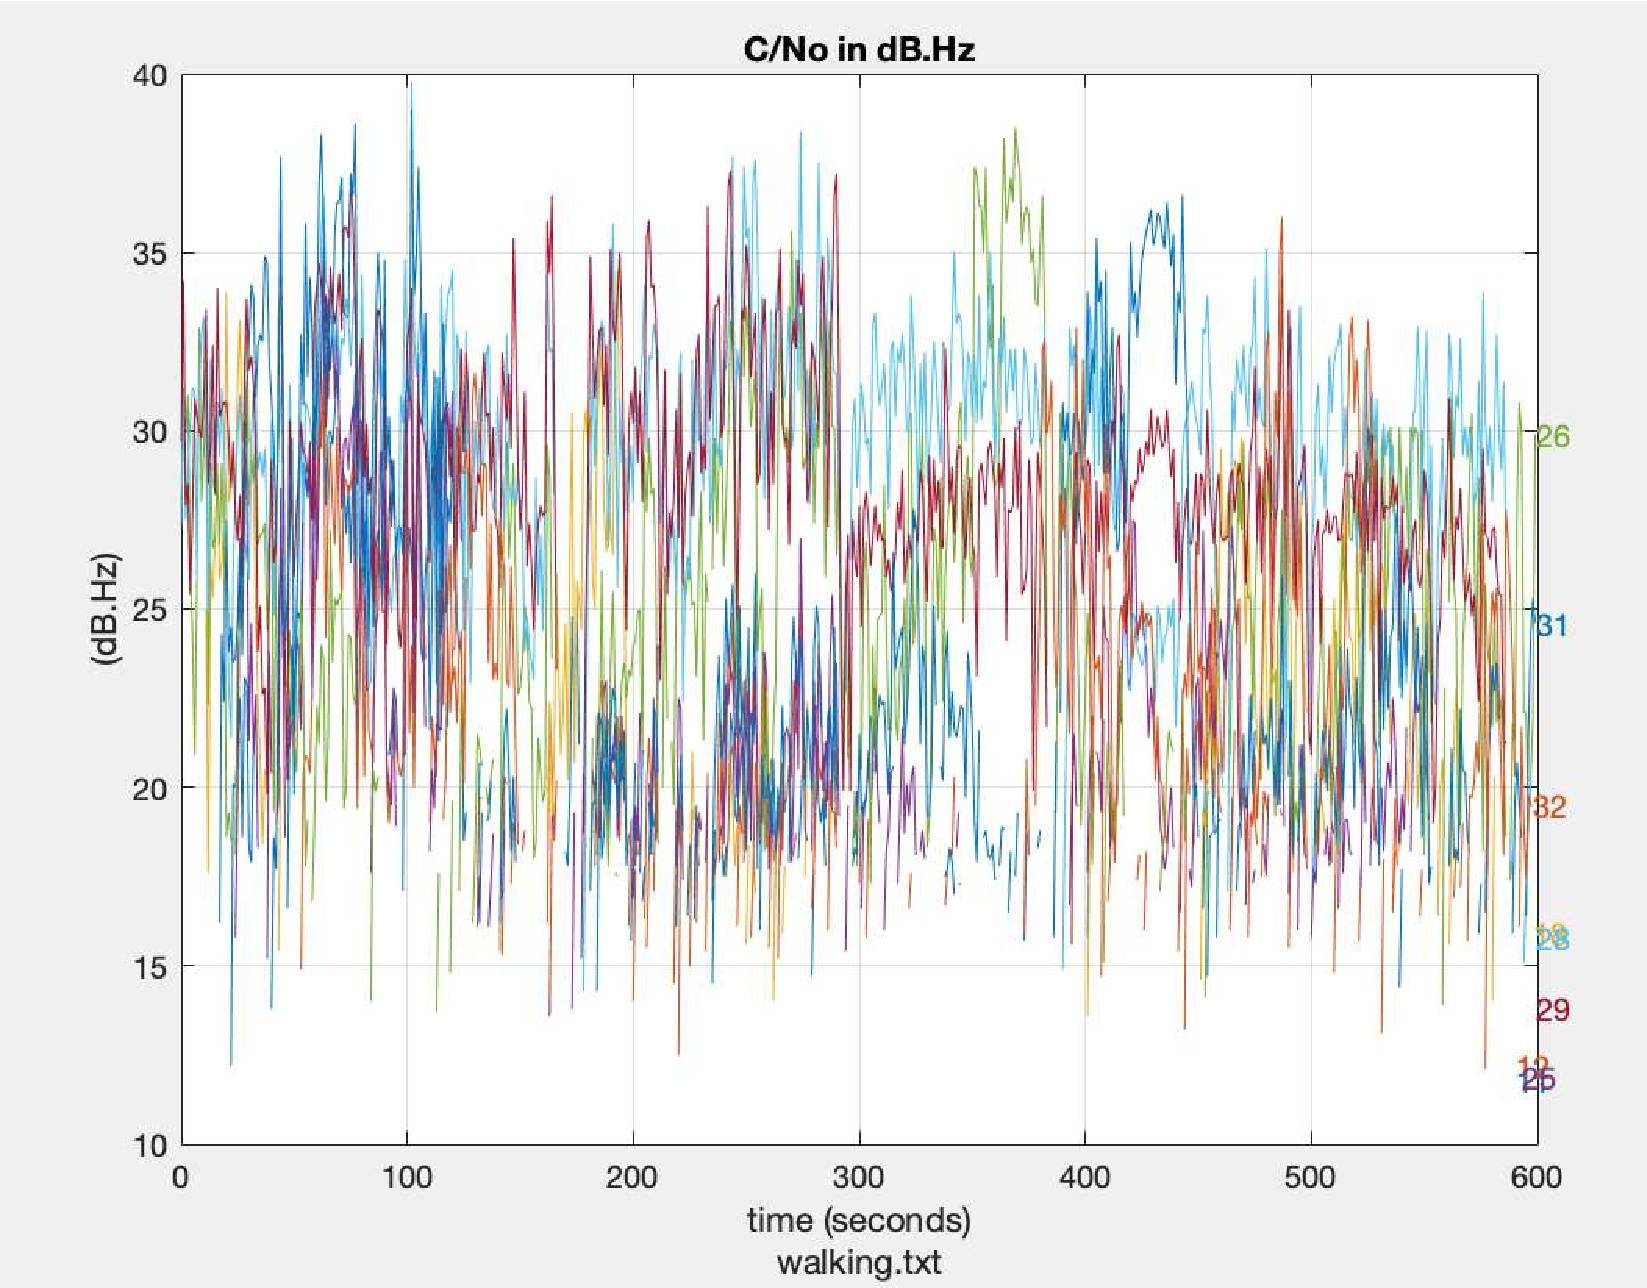
\includegraphics[scale=0.15]{images/walking_figure_3.pdf}
%\caption{C/N0 in dB.Hz}
%\label{fig:figure3_walking}
%\end{figure}
\begin{figure}[H]
  \begin{subfigure}{.22\textwidth}
  \centering
    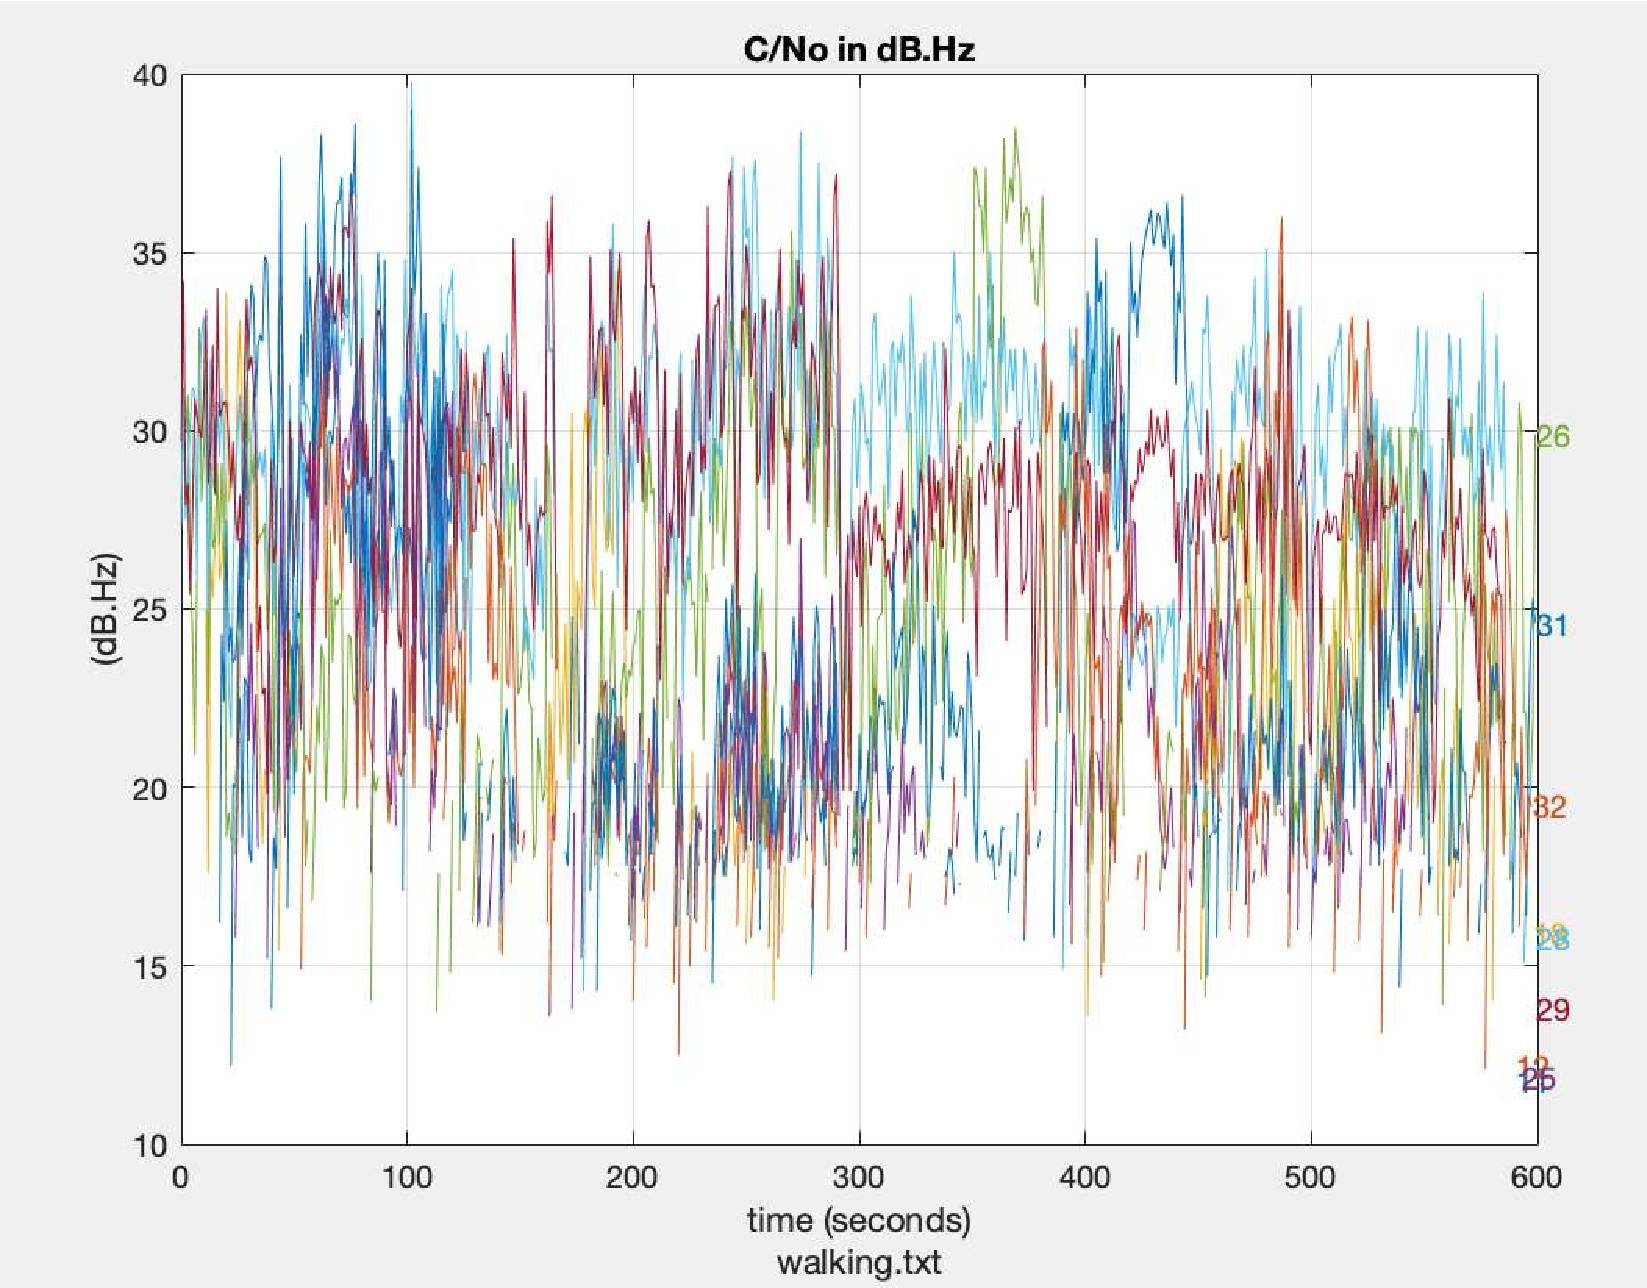
\includegraphics[width=1\linewidth]{images/walking_figure_3.pdf}
    \caption{C/N0 in dB.Hz}
    \label{fig:walking_figure_3.pdf}
  \end{subfigure}
  \begin{subfigure}{.22\textwidth}
  \centering
    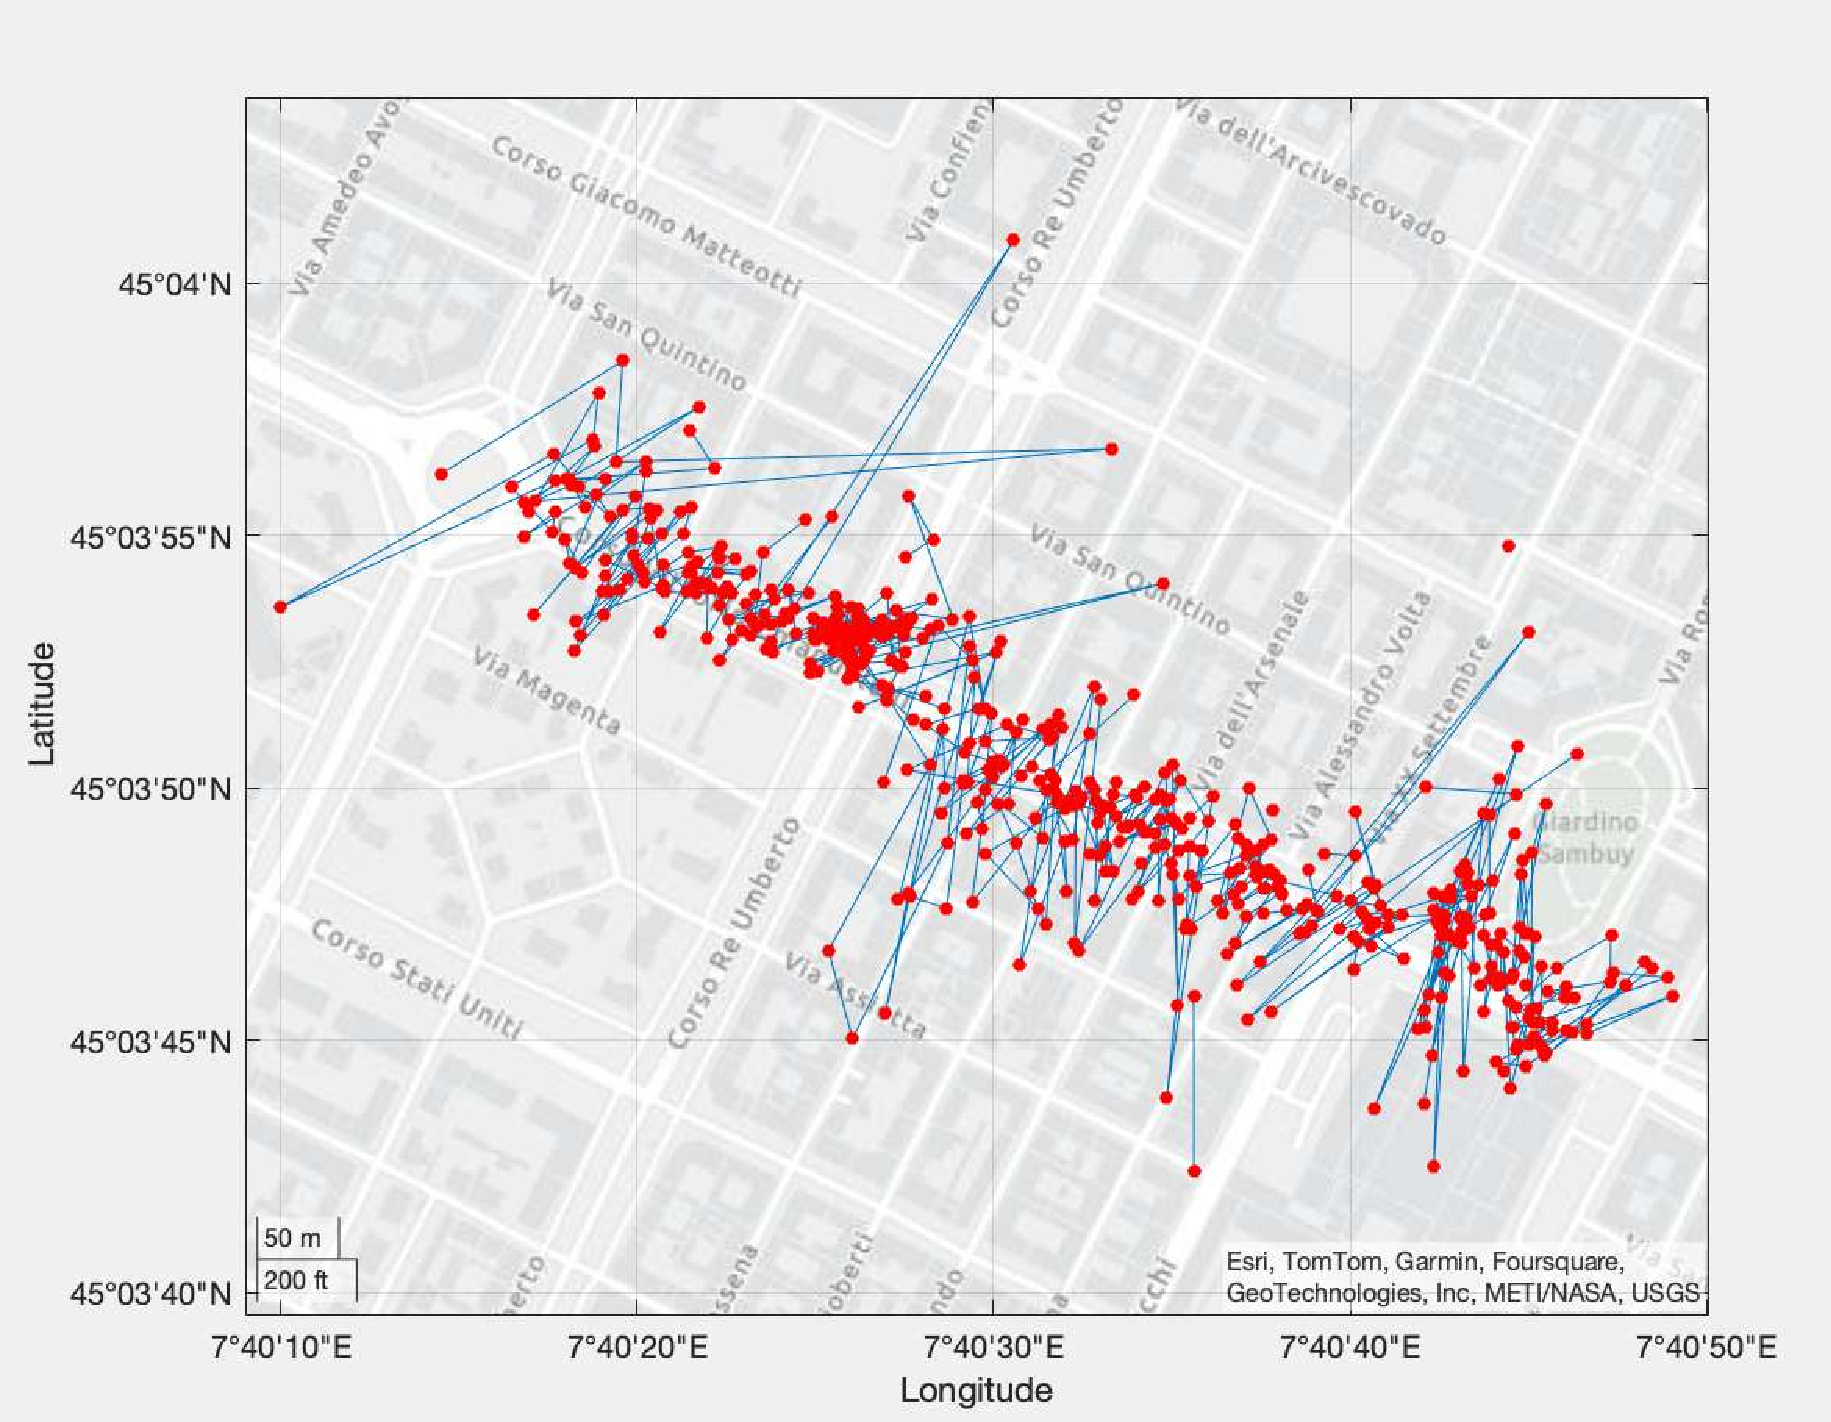
\includegraphics[width=1\linewidth]{images/walking_figure_6.pdf}
    \caption{Positioning solution on map}
    \label{fig:walking_figure_6}
  \end{subfigure}
  \vspace{10pt}
  %\caption{Positioning solution on map}
  %\captionsetup[subfigure]{position=below}
\end{figure}

\subsection{Car}
\label{sec:car}
For this measurement the receiver is located inside a moving car, so the line of sight is partially obstructed. The figure \ref{fig:car_figure_6} shows the receiver's position and we can notice that when the car is inside a tunnel the position is not detected because we cannot get the signals from the satellites. The HDOP value is as good as the open sky measurement. In figure \ref{fig:car_figure_4}, we observe the highest number of satellites in view, which is likely fortuitous, possibly resulting from better satellite geometry at that particular time of measurement. The horizontal speed is mainly distributed between 29 and 31 m/s (about 108 km/h), which is coherent to the speed we had in car since the measurement was performed in highway.
\begin{figure}[H]
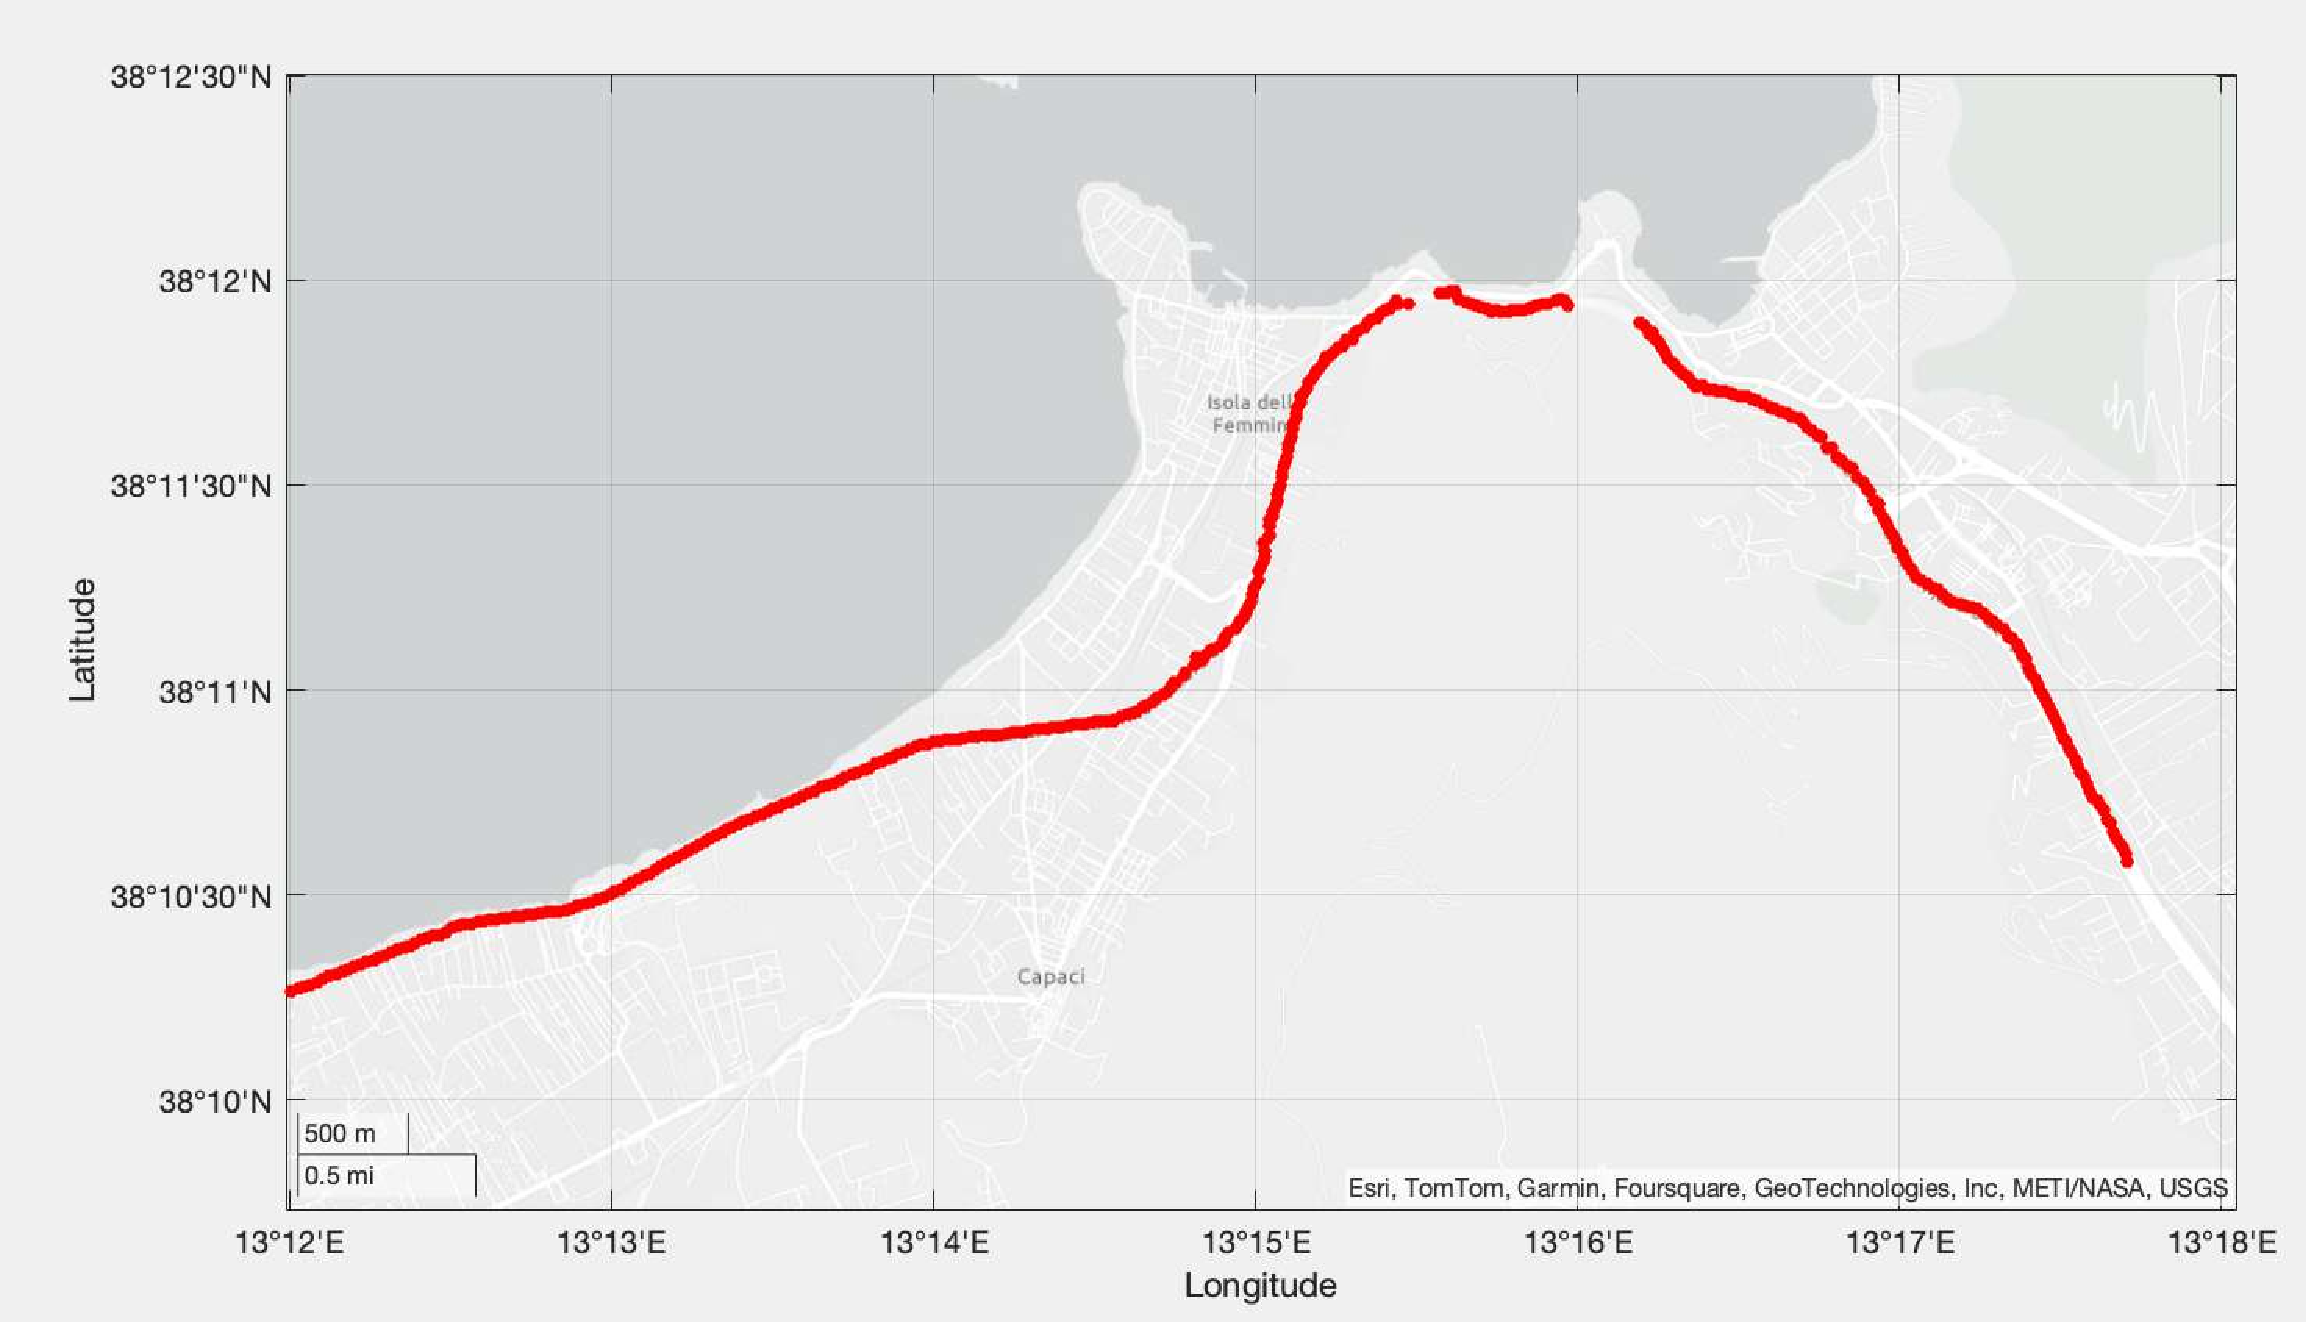
\includegraphics[scale=0.15]{images/car_figure_6.pdf}
\caption{Positioning solution on map}
\label{fig:car_figure_6}
\end{figure}
\begin{figure}[H]
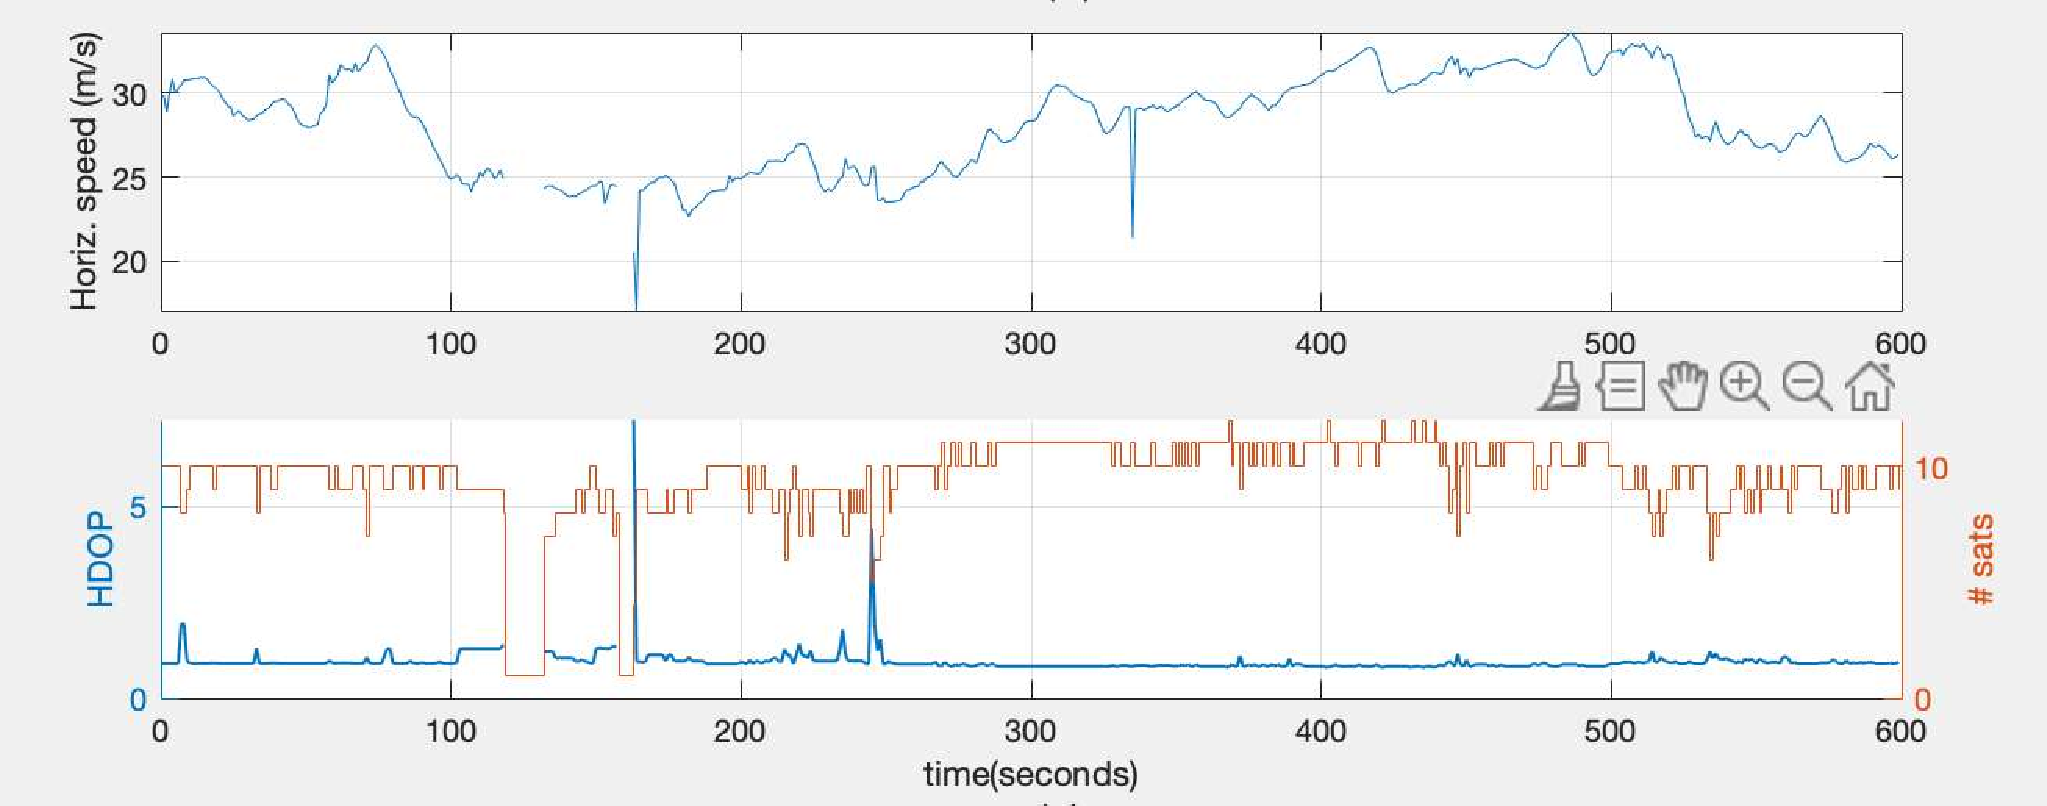
\includegraphics[scale=0.2]{images/car_figure_4.pdf}
\caption{Horizontal speed and HDOP}
\label{fig:car_figure_4}
\end{figure}

%\vspace{0.4cm}

\subsection{Airplane}
\label{sec:airplane}
For this measurement, since the plane can be seen as a Faraday cage, it's fundamental to notice that the only way we can be sure to get signals from satellites is by placing receiver near the window of the airplane. If we are not in the sit near window, we get almost nothing. The figure \ref{fig:airplane_fig_4} shows the rectilinear trajectory of the airplane. We can also notice that in correspondence of a drop of the number of received satellites, we get a spike in HDOP plot. This horizontal speed plot is also useful to understand the speed of the airplane in that moment, which is in a range of 215-240 m/s, and it's plausible because cruise speed of a Boeing 737-800 is about 271 m/s. The figure \ref{fig:airplane_fig_3} shows us that the received signals are quite high, with a C/N0 mean of 29.95 dB.Hz, this may be due to the fact that we have less inferences and obstacles.
\begin{figure}[H]
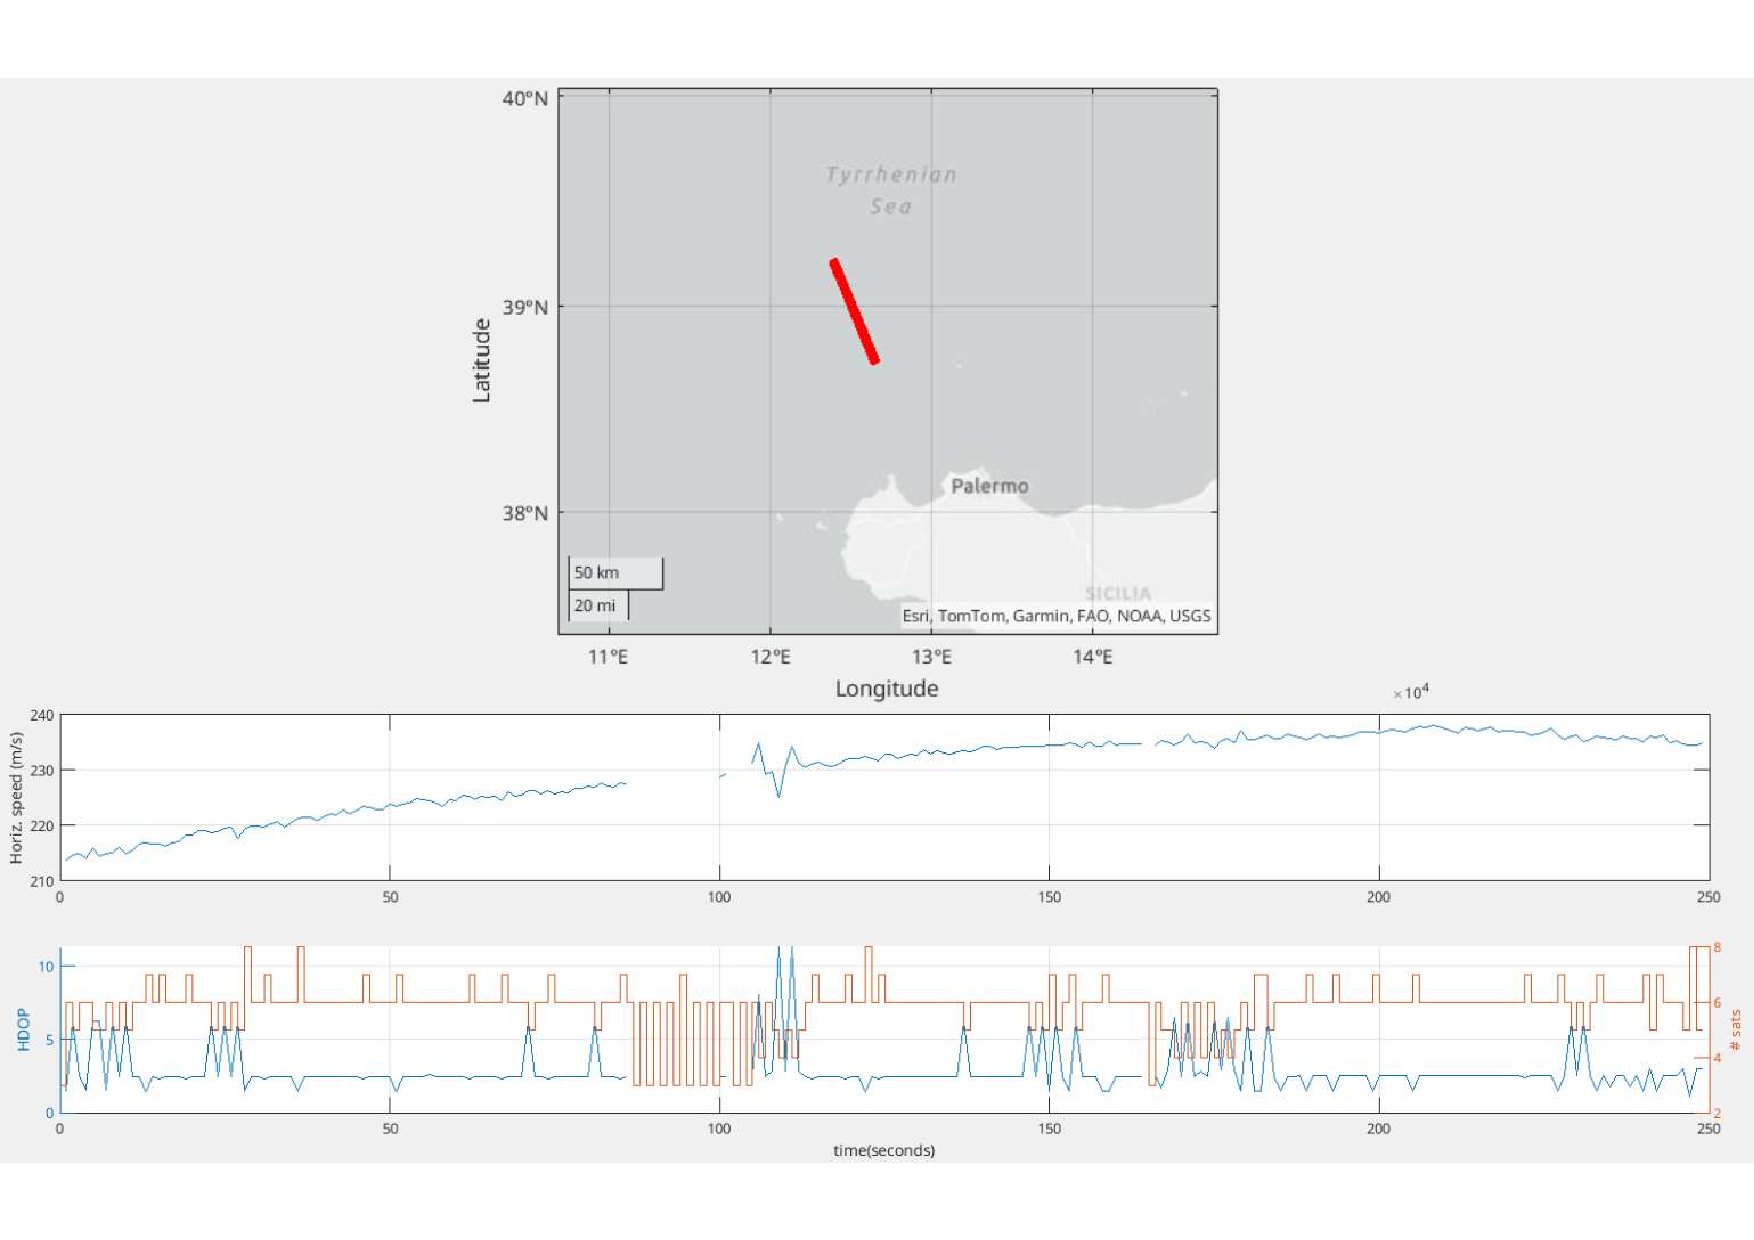
\includegraphics[scale=0.20]{images/airplane_fig_4.pdf}
\caption{Positioning solution on map, Horizontal speed, HDOP}
\label{fig:airplane_fig_4}
\vspace{2pt}
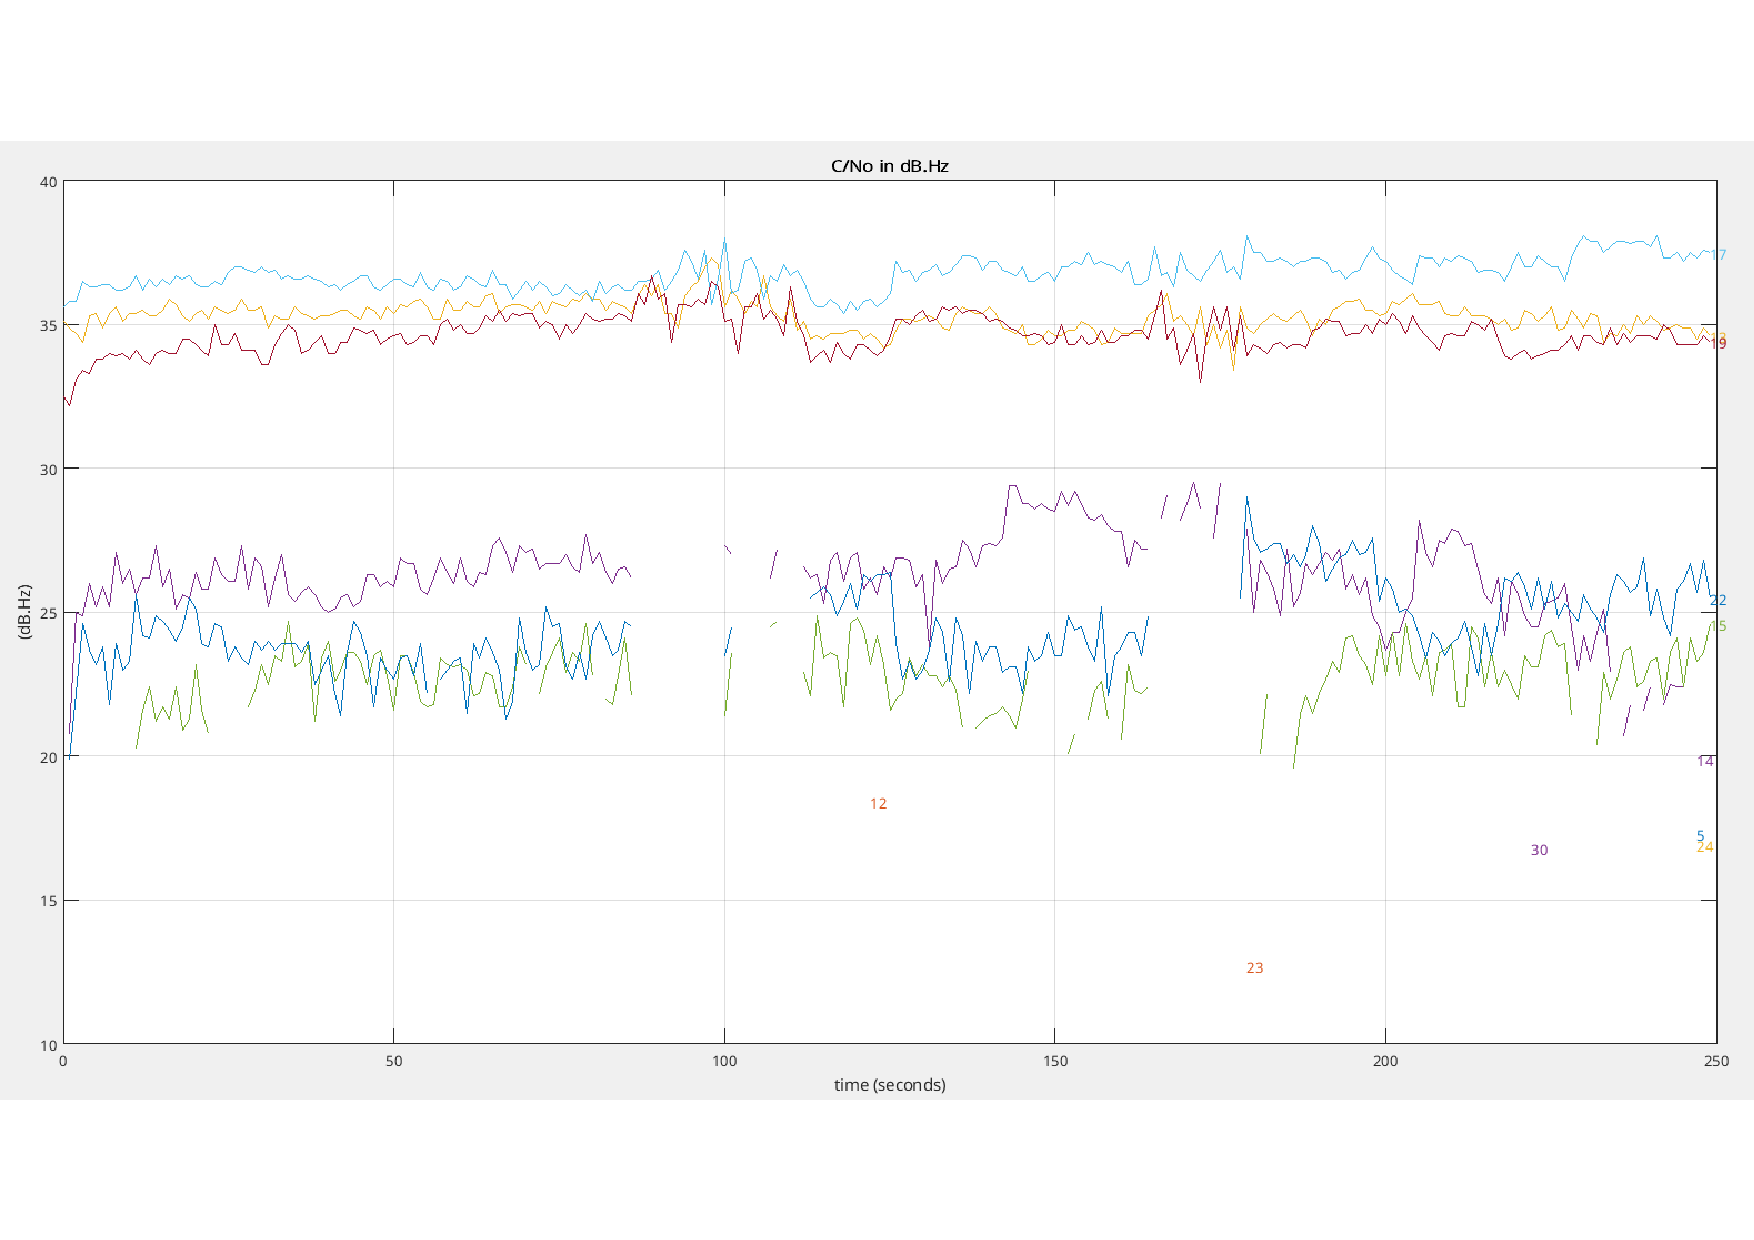
\includegraphics[scale=0.20]{images/airplane_fig_3.pdf}
\caption{C/N0 in dB.Hz}
\label{fig:airplane_fig_3}
\end{figure}
\vspace{0.2cm}